\chapter{Release 2}
\addcontentsline{toc}{chapter}{Release 2}
\markboth{Release 2}{Release 2}
\renewcommand\fbox{\fcolorbox{blue}{white}}
\label{chap:release2}
% section starts from 1 
%\minitoc

\section*{Introduction}

Ce chapitre présente la deuxieme version de notre application.Il est composé de quatre sprints qui ont été réalisés en 8 semaines. Nous avons commencé par l'ajout de la fonctionnalité d'authentification a l'aide en utilisant l'OIDC, puis nous avons ajouté la fonctionnalité de gestion de profile, absence et de delegation. Enfin, nous avons ajouté la fonctionnalité de consultation des statistiques. Dans ce chapitre, nous décrirons en détail les fonctionnalités de chaque sprint, les défis que nous avons rencontrés et les solutions que nous avons apportées pour les surmonter.

Release 2 : (Du 3 Avril au 27 Mai 2023)

\fbox{\begin{minipage}{30em}
  \textbf{Organisation des sprints :} \\
  Cette release contient les quatre sprints:
  \begin{itemize}
    \item \textbf{Sprint 5:} Gestion d'authentification OIDC et verification biometrique.
    \item \textbf{Sprint 6:} Gestion du Profile, d'absence et de délégué.
    \item \textbf{Sprint 7:} Consultation des statistique
    \item \textbf{Sprint 8:} .....
  \end{itemize}
\end{minipage}}

\section{Sprint 7 (Consultation des statistique)}

\subsection{Sprint Goal}
L'objectif de ce sprint est de permettre à l'utilisateur de consulter les statistiques de ses documents et consulter les documents a l'aide de filtre rapide de statistique.

\subsection{Sprint Backlog}


\begin{adjustwidth}{-1cm}{}
  % \usepackage{longtable}
    
    \begin{longtable}{|c|p{6cm}|c|p{6cm}|c|}
      % \centering
      \hline
      \textbf{ID} & \textbf{User story} & \textbf{ID}  & \textbf{Tâche} & \textbf{Durée} \\
      \hline
      \multirow{2}{*}{1} & En tant qu'utilisateur, je veux pouvoir visualiser les statistiques de l'application afin de suivre l'évolution de l'application.
      & 1.1 & Préparer les interfaces sur Figma. & \multirow{3}{*}{2.5 Jour} \\
      \cline{3-4}
      & & 1.2 & Développer le composant de statistique a une valeur. & \\
      \cline{3-4}
      & & 1.3 & Développer le composant de statistique a plusieurs valeurs. & \\
      \cline{3-4}
      & & 1.4 & Développer la fonction qui recuperer et ranger les statistiques. & \\
      & & 1.5 & Développer la fonction qui permet de visualiser les statistiques. & \\
      % & & 1.6 & Développer la fonction qui permet de filtrer les documents par statistique. & \\
      \cline{1-5}
      \multirow{2}{*}{2} & En tant qu'utilisateur, je veux pouvoir consulter les documents a l'aide de filtre rapide afin de trouver les documents que je cherche. & 2.1.& Ajouter la fonction de filtre a l'interface de consultation des statistiques. & \multirow{2}{*}{0.5 Jour} \\
      \cline{3-4}
      & & 2.2 & Développer la fonction qui permet de filtrer les documents par statistique. & \\
      \cline{1-5}
      \multirow{2}{*}{3} & En tant qu'utilisateur, je veux pouvoir refraichir les données de l'application afin de voir les dernières informations. & 3.1.& Ajouter l'interface de rafraichissement des données a chaque page possible. & \multirow{2}{*}{0.5 Jour} \\
      \cline{3-4}
      & & 3.2 & Développer la fonction qui permet de rafraichir les données de chaque page. & \\
      \cline{1-5}
  \hline
  \caption{Sprint backlog du Sprint 5}
  \label{tab:sprint-backlog-5}
\end{longtable}
\end{adjustwidth}


\subsection{Implémentation du Sprint 5}
\textbf{•	Diagramme de cas d'utilisation du sprint 5}

% add image
\begin{figure}[H]
  \centering
  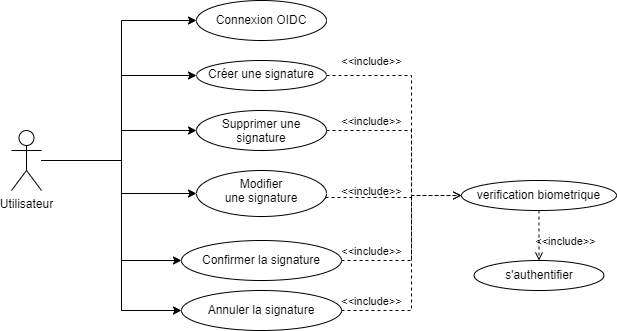
\includegraphics[width=0.8\textwidth]{use_case_sprint_5}
  \caption{Diagramme de cas d'utilisation du sprint 5}
  \label{fig:UseCaseDiagramSp51}
\end{figure}

\subsubsection{Analyse des besoins:}
\textbf{•	Description textuelle de cas d'utilisation « Consulter les statistiques »}

\begin{longtable}{|p{5cm}|p{10cm}|}
\hline
\textbf{Cas d'utilisation}&Consulter les statistiques\\
\hline
\textbf{Acteurs}&Utilisateur\\
\hline
\textbf{Pré Condition}&L'utilisateur est authentifié\\
\hline
\textbf{Post Condition}&Consultation des statistiques\\
\hline
\textbf{Scénario Nominal}&
\vspace{-\baselineskip}
\begin{enumerate}
  \setcounter{enumi}{1}
      \item [2.1] L'utilisateur clique sur le bouton « Accueil »
      \item [2.2] Le système affiche les statistiques
\end{enumerate}\\
\hline
\textbf{Scénario d'exception}&Erreur de connexion\\
\hline
\caption{Description textuelle du diagramme de cas d'utilisation « Consulter les statistiques »}
\label{tab:use_case_consulter_statistiques}
\end{longtable}

\textbf{•	Description textuelle de cas d'utilisation « Consulter les documents a l'aide de filtre rapide »}

\begin{longtable}{|p{5cm}|p{10cm}|}
\hline
\textbf{Cas d'utilisation}&Consulter les documents a l'aide de filtre rapide\\
\hline
\textbf{Acteurs}&Utilisateur \\
\hline
\textbf{Pré Condition}&L'utilisateur doit être authentifié\\
\hline
\textbf{Post Condition}&Consultation des documents a l'aide de filtre rapide\\
\hline
\textbf{Scénario Nominal}&
\vspace{-\baselineskip}
\begin{enumerate}
    \setcounter{enumi}{1}
      \item L'utilisateur clique sur l'une des widget
      \item Le système affiche les documents correspondant au filtre
\end{enumerate}\\
\hline
\textbf{Scénario d'exception}&Erreur de connexion\\
\hline
\caption{Description textuelle du diagramme de cas d'utilisation « Consulter les documents a l'aide de filtre rapide »}
\label{tab:use_case_consulter_documents_filtre_rapide}
\end{longtable}

\begin{figure}[H]
  \centering
  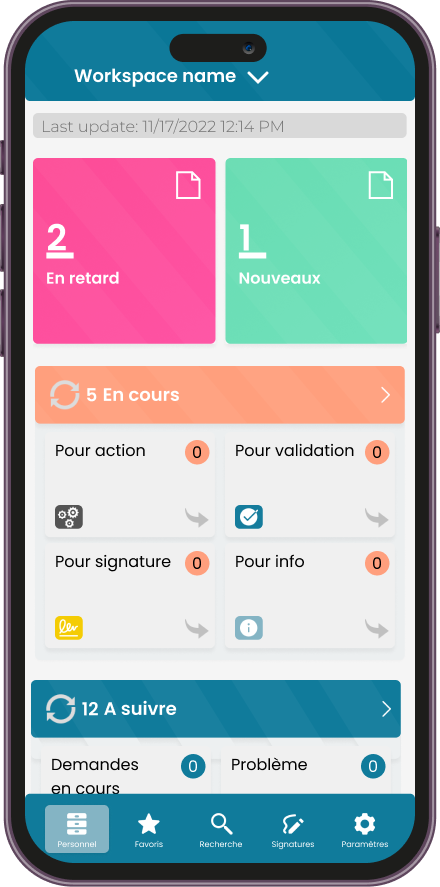
\includegraphics[width=0.7\textwidth]{design_statistique}
  \caption{Maquette de la page de statistique}
  \label{fig:design_statistique}
\end{figure}


Pour avoir une représentation temporelle des interactions entre les objets de notre système et de la chronologie des messages échangés entre eux et avec les acteurs nous avons réalisé les diagrammes de séquence représentés ci-dessous

\begin{figure}[H]
  \centering
  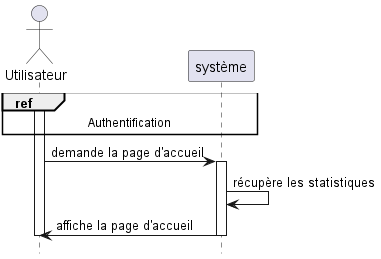
\includegraphics[width=0.7\textwidth]{out/diagrams/sprint5/view_stats/view_stats}
  \caption{Diagramme de séquence de cas d'utilisation « Consulter les statistiques »}
  \label{fig:sequence_view_stats}
\end{figure}

\begin{figure}[H]
  \centering
  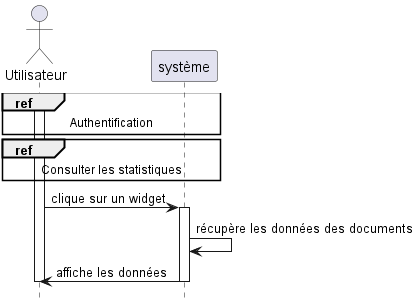
\includegraphics[width=0.7\textwidth]{out/diagrams/sprint5/docs_quick_filter/docs_quick_filter}
  \caption{Diagramme de séquence de cas d'utilisation « Consulter les documents a l'aide de filtre rapide »}
  \label{fig:sequence_docs_quick_filter}
\end{figure}


\subsubsection{Analyse détaillée}
La présentation de démarche d'analyse fonctionnelle d'un sprint est très importante pour la satisfaction d'un client parce qu'elle consiste à caractériser les fonctions offertes par un produit.
Donc, nous allons faire l'analyse des différents cas d'utilisation en utilisant le diagramme de classes d'analyse.


% spacing between paragraphs
\setlength{\parskip}{1em}
% spacing left
\setlength{\parindent}{0em}

\textbf{•	Diagramme de classe d'analyse de sprint 5 }


\begin{figure}[H]
  \centering
  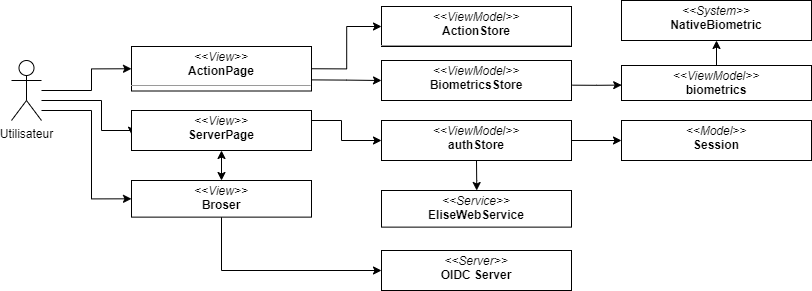
\includegraphics[width=1\textwidth]{dca_sprint5}
  \caption{Diagramme de classe d'analyse de sprint 5}
  \label{fig:class_analyse_sprint5}
\end{figure}


\subsubsection{Conception}

Après la présentation des diagrammes d'analyse, nous avons présenté dans cette partie les diagrammes de conception.\\ 
Nous allons présenter dans cette partie les diagrammes de conception de sprint 5. \\
\textbf{•	Diagramme de classe de conception de sprint 5}

% add image
\begin{figure}[H]
  \centering
  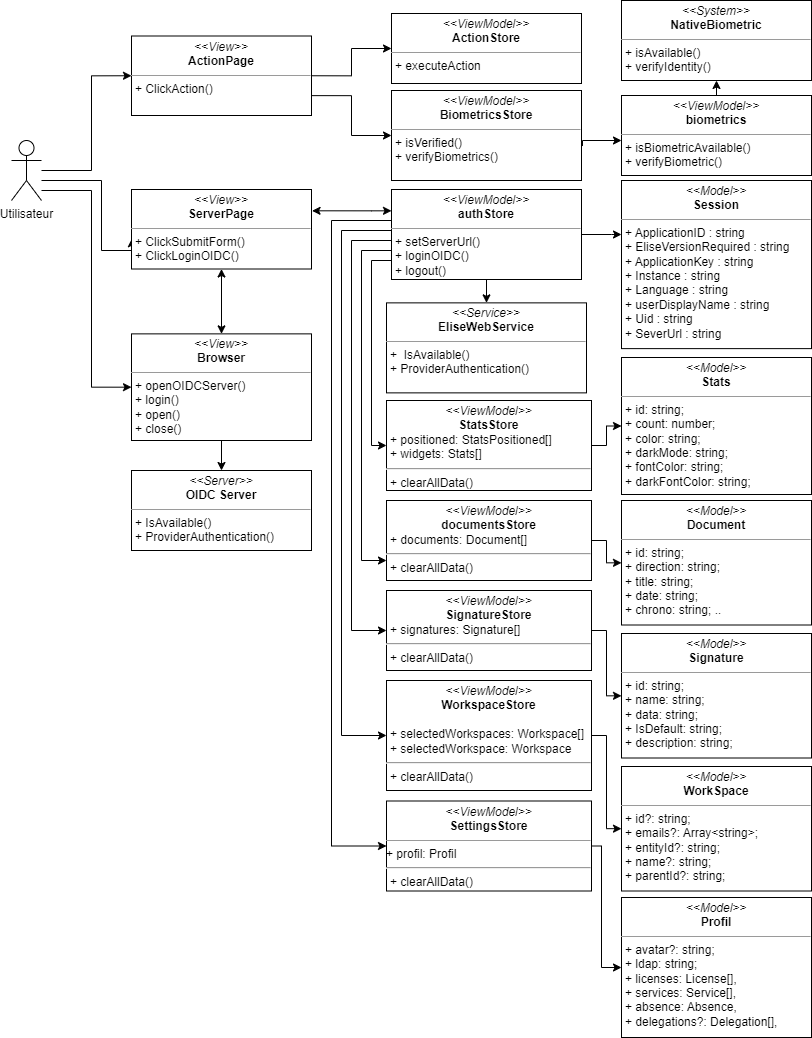
\includegraphics[width=1\textwidth]{dcc_sprint5}
  \caption{Diagramme de classe de conception de sprint 5}
  \label{fig:class_diagram_5}
\end{figure}


% \begin{figure}[H]
%   \centering
%   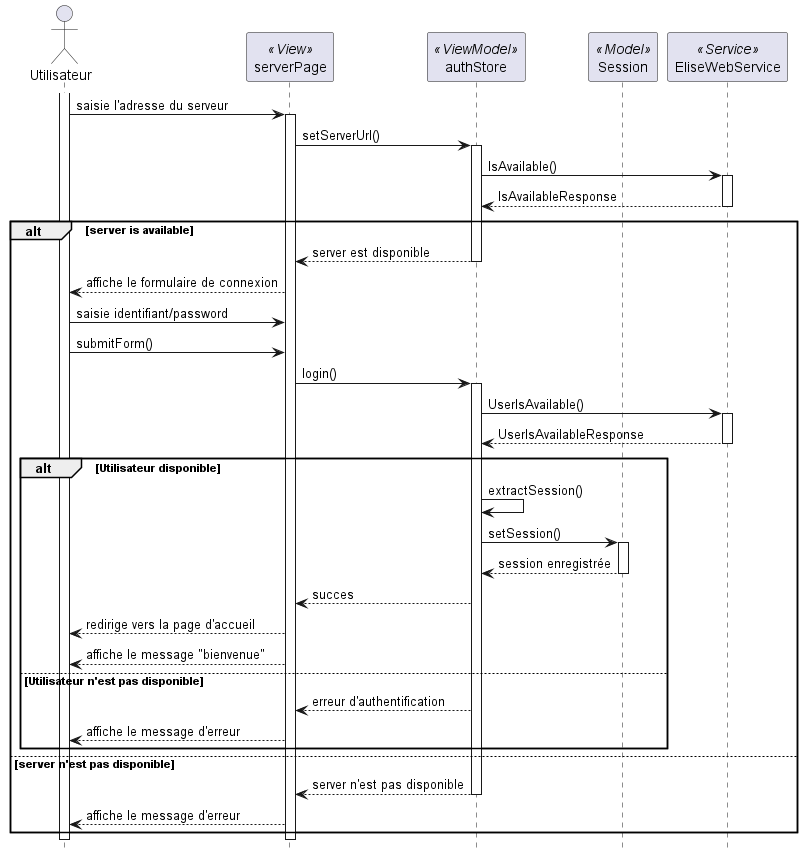
\includegraphics[width=1\textwidth]{out/diagrams/authentification/sequence_simple_login/sequence_simple_login}
%   \caption{Diagramme de séquence de conception de cas d'utilisation « S'authentifier »}
%   \label{fig:sequence_conception_login}
% \end{figure}

% \begin{figure}[H]
%   \centering
%   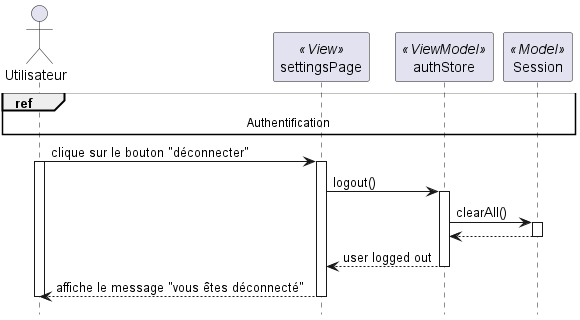
\includegraphics[width=1\textwidth]{out/diagrams/authentification/sequence_logout/sequence_logout}
%   \caption{Diagramme de séquence de conception de cas d'utilisation « Se déconnecter »}
%   \label{fig:sequence_conception_logout}
% \end{figure}

\subsubsection{Réalisation}

Après la présentation des diagrammes d'analyse, nous avons présenté dans cette partie des captures d'écran de l'application.

% add image
\begin{figure}[H]
  \centering
  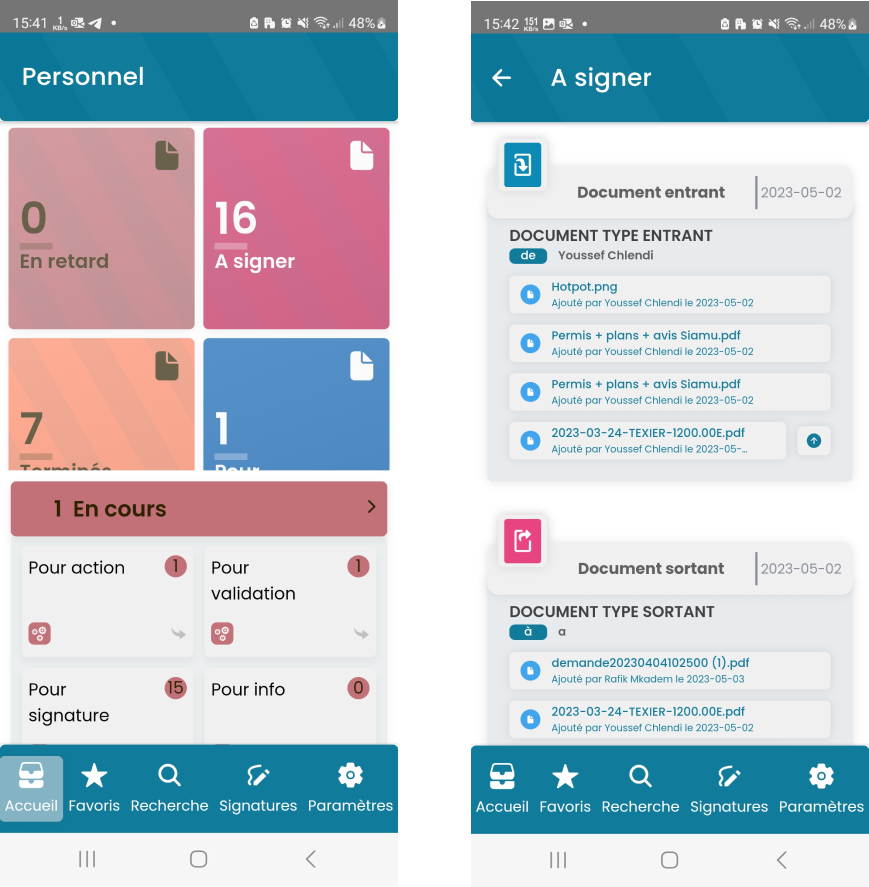
\includegraphics[width=0.7\textwidth, height=0.7\textheight,keepaspectratio=true]{realisation_sprint5}
  \caption{Les interfaces de consultation des statistiques et des documents à l'aide de filtre rapide}
  \label{fig:realisation_sprint5}
\end{figure}

\subsection{Sprint Review}
Suite à cette Technical Story, nous avons préparé notre environnement de travail où nous aurons les possibilités de traiter les prochains sprints.

\subsection{Sprint Retrospective}

\begin{itemize}
  \item \textbf{Ce qui a bien fonctionné :}
  \begin{itemize}
    \item Nous avons pu suivre les formations préparées par la société.
    \item Nous avons pu suivre les formations sur Youtube.
    \item Nous avons pu installer les outils nécessaires pour le développement.
    \item Nous avons bien mis nos connaissances en pratique dans certains projets préparatoires (Application 1, 2, 3 et 4).
    \item Nous avons pu bien initialiser le projet.
    \item Nous avons pu développer la fonctionnalité d'authentification.
  \end{itemize}
  \item \textbf{Ce qui n'a pas bien fonctionné :}
  
  Nous avons remarqué que le temps de formation est très réduit, nous avons donc décidé de suivre des formations sur Youtube pour nous former sur les technologies à utiliser en plus de la formation préparée par la société.
\end{itemize}
